\chapter{Financial Planning and Investment}\label{ch:financial-planning}

I remember sitting with a talented entrepreneur from Boston who had an innovative AgriTech solution. ``Dele,'' he said, pulling out an impressively detailed financial model, ``I've planned everything down to the last naira.'' Looking at his numbers, I couldn't help but smile --- he's thinking \$500,000 for his initial entry when he could have started effectively with \$75,000.

``Let me share something I learned while building Firmbird,'' I told him. ``In Nigeria, it's not about how much money you start with --- it's about how smartly you deploy it.''

\begin{importantbox}
When I shared that entrepreneur revise his plan, he ended up entering the market with a lot, lot less and achieved profitability in 11 months.\ This chapter will show you how to plan your finances similarly --- efficiently and realistically.
\end{importantbox}

\section{Smart Money: Right-Sizing Your Investment}\label{sec:smart-money}

Let's start with what I call the ``Minimal Viable Investment'' (MVI) approach. This isn't about being cheap; it's about being smart with your capital. Here's what I've seen work consistently across different sectors:

\begin{center}
\begin{tabularx}{\textwidth}{>{\raggedright\arraybackslash}X >{\centering\arraybackslash}X >{\raggedright\arraybackslash}X}
    \toprule
    \textbf{Business Type} & \textbf{Minimum Capital} & \textbf{Key Allocations} \\
    \midrule
    Tech Startup & \$50,000 & Infrastructure, development, minimal team \\
    Retail/Trade & \$75,000 & Stock, storage, basic operations \\
    Professional Services & \$30,000 & Office setup, licensing, marketing \\
    Light Manufacturing & \$100,000 & Equipment, workspace, initial materials \\
    \bottomrule
\end{tabularx}
\end{center}

\section{The Real Cost Structure}\label{sec:real-cost-structure}

When a UAE-based client asked about setup costs, I drew what I now call the ``Cost Triangle'':

\begin{figure}[h]
    \centering
    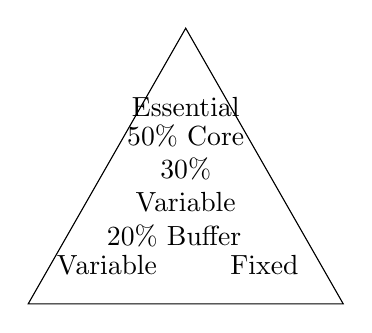
\begin{tikzpicture}
        % Cost Triangle visualization
        \draw (0,0) -- (4,0) -- (2,3.5) -- cycle;
        \node at (2,2.5) {Essential};
        \node at (1,0.5) {Variable};
        \node at (3,0.5) {Fixed};
        % Add percentages
        \node[text width=2cm] at (2,1.5) {\centering 50\% Core\\30\% Variable\\20\% Buffer};
    \end{tikzpicture}
    \caption{The Cost Triangle Framework}
    \label{fig:cost-triangle}
\end{figure}

Let's break this down into practical terms:

\subsection{Essential Setup Costs}\label{subsec:essential-setup-costs}
These are your non-negotiable startup expenses:

\begin{tcolorbox}[colback=white,colframe=primarydark,title=\textbf{Core Setup Components}]
\begin{itemize}
    \item \textbf{Legal \& Registration: \$5,000}
    \begin{itemize}
        \item Company registration
        \item Basic licenses
        \item Initial compliance
    \end{itemize}

    \item \textbf{Infrastructure: \$10,000-30,000}
    \begin{itemize}
        \item Office space (if needed)
        \item Basic equipment
        \item Utilities setup
    \end{itemize}

    \item \textbf{Technology: \$5,000-20,000}
    \begin{itemize}
        \item Core systems
        \item Essential software
        \item Basic security
    \end{itemize}

    \item \textbf{Initial Team: \$3,000-8,000}
    \begin{itemize}
        \item Essential personnel
        \item Basic training
        \item Initial payroll buffer
    \end{itemize}
\end{itemize}
\end{tcolorbox}

\section{Monthly Operating Costs}\label{sec:monthly-operating-costs}

I always tell entrepreneurs, ``Your first three months of operating costs aren't a cost --- they're part of your startup capital.'' Here's why:

\begin{center}
\begin{tabularx}{\textwidth}{>{\raggedright\arraybackslash}X >{\centering\arraybackslash}X >{\raggedright\arraybackslash}X}
    \toprule
    \textbf{Expense Category} & \textbf{Monthly Range} & \textbf{Notes} \\
    \midrule
    Staff & \$2,000-4,000 & Start lean, scale with revenue \\
    Infrastructure & \$1,500-3,000 & Location dependent \\
    Technology & \$500-1,500 & Based on business type \\
    Marketing & \$1,000-2,000 & Focus on targeted efforts \\
    Miscellaneous & \$500-1,000 & Always have a buffer \\
    \bottomrule
\end{tabularx}
\end{center}

\section{Revenue Projection Framework}\label{sec:revenue-projection}

A UK founder once asked me, ``Dele, how do I project revenues in a market I don't fully understand yet?'' I introduced her to what I call the ``Conservative Growth Ladder'':

\begin{tcolorbox}[colback=white,colframe=primarydark,title=\textbf{12-Month Revenue Framework}]
\begin{itemize}
    \item \textbf{Months 1--3: Establishment Phase}
    \begin{itemize}
        \item Focus on setup and initial clients
        \item Expect minimal revenue
        \item Target: Cover 20--30\% of operating costs
    \end{itemize}

    \item \textbf{Months 4-6: Growth Phase}
    \begin{itemize}
        \item Expand client base
        \item Optimize operations
        \item Target: Cover 50-60\% of operating costs
    \end{itemize}

    \item \textbf{Months 7-9: Stabilization Phase}
    \begin{itemize}
        \item Strengthen market position
        \item Increase efficiency
        \item Target: Cover 80-90\% of operating costs
    \end{itemize}

    \item \textbf{Months 10-12: Profitability Phase}
    \begin{itemize}
        \item Achieve stable operations
        \item Focus on profitability
        \item Target: Break-even or slight profit
    \end{itemize}
\end{itemize}
\end{tcolorbox}

\section{Sector-Specific Considerations}\label{sec:sector-specific}

Let me share what I call the ``Sector Success Formula'' --- key financial focuses for different business types:

\subsection{Technology Sector}\label{subsec:technology-sector}
\begin{tcolorbox}[colback=white,colframe=primary,title=\textbf{Tech Sector Financial Focus}]
\begin{itemize}
    \item \textbf{Development Costs: \$20,000-30,000}
    \begin{itemize}
        \item MVP development
        \item Testing and iteration
        \item Initial infrastructure
    \end{itemize}

    \item \textbf{Market Entry: \$15,000-20,000}
    \begin{itemize}
        \item User acquisition
        \item Market validation
        \item Initial scaling
    \end{itemize}
\end{itemize}
\end{tcolorbox}

\subsection{Retail/Trade}\label{subsec:retail-trade}
\begin{tcolorbox}[colback=white,colframe=primary,title=\textbf{Retail/Trade Financial Focus}]
\begin{itemize}
    \item \textbf{Inventory: \$30,000-40,000}
    \begin{itemize}
        \item Initial stock
        \item Storage solutions
        \item Supply chain setup
    \end{itemize}

    \item \textbf{Operations: \$20,000-25,000}
    \begin{itemize}
        \item Location setup
        \item Staff hiring
        \item Systems implementation
    \end{itemize}
\end{itemize}
\end{tcolorbox}

\subsection{Professional Services}\label{subsec:professional-services}
\begin{tcolorbox}[colback=white,colframe=primary,title=\textbf{Services Sector Financial Focus}]
\begin{itemize}
    \item \textbf{Setup: \$15,000-20,000}
    \begin{itemize}
        \item Office establishment
        \item Professional certifications
        \item Initial marketing
    \end{itemize}

    \item \textbf{Operations: \$10,000-15,000}
    \begin{itemize}
        \item Core team
        \item Basic systems
        \item Network building
    \end{itemize}
\end{itemize}
\end{tcolorbox}

\section{Funding Sources and Strategies}\label{sec:funding-sources}

When it comes to funding your Nigerian market entry, I always share what I call the ``4S Framework'':

\begin{center}
\begin{tabularx}{\textwidth}{>{\raggedright\arraybackslash}X >{\centering\arraybackslash}X >{\raggedright\arraybackslash}X}
    \toprule
    \textbf{Source} & \textbf{Typical Range} & \textbf{Best For} \\
    \midrule
    Self-Funding & \$30,000-100,000 & Quick start, full control \\
    Silent Partners & \$50,000-200,000 & Expanded capacity \\
    Strategic Investors & \$100,000-500,000 & Market access \\
    Staged Investment & \$50,000-150,000 & Risk management \\
    \bottomrule
\end{tabularx}
\end{center}

\begin{warningbox}
I've seen too many entrepreneurs get caught in what I call the ``Big Money Trap'' --- raising more than they need and losing focus.\ Start with what you need, not what you can get.
\end{warningbox}

\section{Interactive Financial Planning Tools}\label{sec:financial-tools}

To help you plan your finances more effectively, we've created an interactive financial planning calculator.\ This tool will help you:

\begin{itemize}
    \item Model different scenarios
    \item Understand cost breakdowns
    \item Project cash flows
    \item Plan contingencies
\end{itemize}

You can access this tool at \texttt{https://circle.counseal.com}

\section{Workshop: Your Financial Plan}\label{sec:workshop}

\begin{workshopbox}
\textbf{Financial Planning Exercise}

1. Capital Requirements
\begin{itemize}
    \item Core setup costs: \_\_\_\_\_\_\_\_\_
    \item Operating buffer: \_\_\_\_\_\_\_\_\_
    \item Growth capital: \_\_\_\_\_\_\_\_\_
\end{itemize}

2. Monthly Budget
\begin{itemize}
    \item Fixed costs: \_\_\_\_\_\_\_\_\_
    \item Variable costs: \_\_\_\_\_\_\_\_\_
    \item Revenue targets: \_\_\_\_\_\_\_\_\_
\end{itemize}

3. Funding Strategy
\begin{itemize}
    \item Primary source: \_\_\_\_\_\_\_\_\_
    \item Backup options: \_\_\_\_\_\_\_\_\_
    \item Staged planning: \_\_\_\_\_\_\_\_\_
\end{itemize}
\end{workshopbox}

\begin{communitybox}
Connect with fellow entrepreneurs and access additional resources on the Africa Growth Circle:
\begin{itemize}
    \item Financial modeling templates
    \item Budgeting tools
    \item Funding source directory
    \item Expert advisory sessions
\end{itemize}
Visit circle.counseal.com to join the conversation.
\end{communitybox}

\begin{importantbox}
Remember, successful market entry isn't about having the most money --- it's about having enough money and using it wisely.\ In the next chapter, we'll explore how to protect your investment through effective risk management and compliance.
\end{importantbox}
